\documentclass{article}
\usepackage[utf8]{inputenc}

\title{KREPE-2 Avionics Documentation}
\author{Matt Ruffner}
\date{}

\usepackage{url}
\usepackage{float}
\usepackage{natbib}
\usepackage{graphicx}
\usepackage{listings}
\usepackage{fullpage}
\usepackage{hyperref}
\hypersetup{
    colorlinks=true,
    linkcolor=blue,
    filecolor=magenta,      
    urlcolor=cyan,
}

\begin{document}

\maketitle
\tableofcontents
\listoffigures
\listoftables
\newpage


%%%%%%%%%%%%%%%%%%%%%%%%%%%%%%%%%%%%%%%%%%%%%%%%%%%%%%%%%%%%%%%%%%%%%%%%%%%%%%%%%%%%%%%%%
%%%%%%%%%%%%%%%%%%%%%%%%%%%%%%%%%%%%%%%%%%%%%%%%%%%%%%%%%%%%%%%%%%%%%%%%%%%%%%%%%%%%%%%%%
%%%%%%%%%%%%%%%%%%%%%%%%%%%%%%%%%%%%%%%%%%%%%%%%%%%%%%%%%%%%%%%%%%%%%%%%%%%%%%%%%%%%%%%%%
%%%%%%%%%%%%%%%%%%%%%%%%%%%%%%%%%%%%%%%%%%%%%%%%%%%%%%%%%%%%%%%%%%%%%%%%%%%%%%%%%%%%%%%%%
\section{Introduction}

This document contains information about the flight computer for the KREPE mission as well as the safety precautions taken to ensure the flight hardware is not a danger to the ISS or its astronauts. In addition to electrical designs and schematics, this document contains pin names, links to datasheets, and implementation notes. The following sections outline the subsystems of the flight computer, pin names for software usage, and datasheets. Other details about the power subsystem including battery type and rating are also included. 

The entire flight ready assembly is referred to as KREPE, which consists of a capsule containing the science (flight computer, batteries, etc.) and a metal shell known as KREM that acts as a Faraday cage, inhibiting any inadvertent RF radiation from the capsule. Both primary and secondary activation must occur for the capsule to become fully active and begin RF transmissions. To avoid accidental activation of hazardous subsystems, secondary activation criteria must be met. Primary and secondary activation processes are discussed in sections ~\ref{sec:primary-activation},\ref{sec:secondary-activation}, and \ref{sec:radio-power-control}.

The subsystems of the flight computer are outlined in Sec.~\ref{sec:subsystems}. Pin definitions are listed with each hardware or sensor component along with any relevant information regarding safety or implementation. Electrical schematics, microcontroller reference cards, and a partslist are shown in  Appendices ~\ref{appa}, \ref{app:pinmap}, and \ref{app:partslist}, respectively.


\subsection{Primary Activation}
\label{sec:primary-activation}
Primary activation is triggered by a pin pulled out of KREPE by astronauts. Once the pin is pulled, a mechanical switch\footnote{\url{https://www.digikey.com/product-detail/en/omron-electronics-inc-emc-div/D2SW-3L1H/Z12268-ND/1811989}} is closed and the flight computer boots to dormant mode where it consumes minimal power. The Iridium radio is not powered on in dormant mode. After pulling the pull tab, a piece of copper tape is put over the hole and primary activation is the complete. Copper tape ensures the KREM is completely sealed with regard to EMI. 

A schematic showing battery protection and primary activation circuitry activation is shown in Fig. \ref{fig:activation-circuitry}. Less than 5 inches of copper 20 AWG PVC insulated wire is used to connect the batteries to the first power function (battery protection circuitry).


%The \texttt{POWER\_SW} header must closed for protected battery or USB voltage to be applied to the Teensy's VIN pin, powering on the system. The location of these connection points can be seen in Fig. \ref{fig:board-top} labelled on the silk screen in the left middle of the PCB. A rendering of the bottom of the board is shown in Fig. \ref{fig:board-bottom}.


\begin{figure}[H]
    \centering
    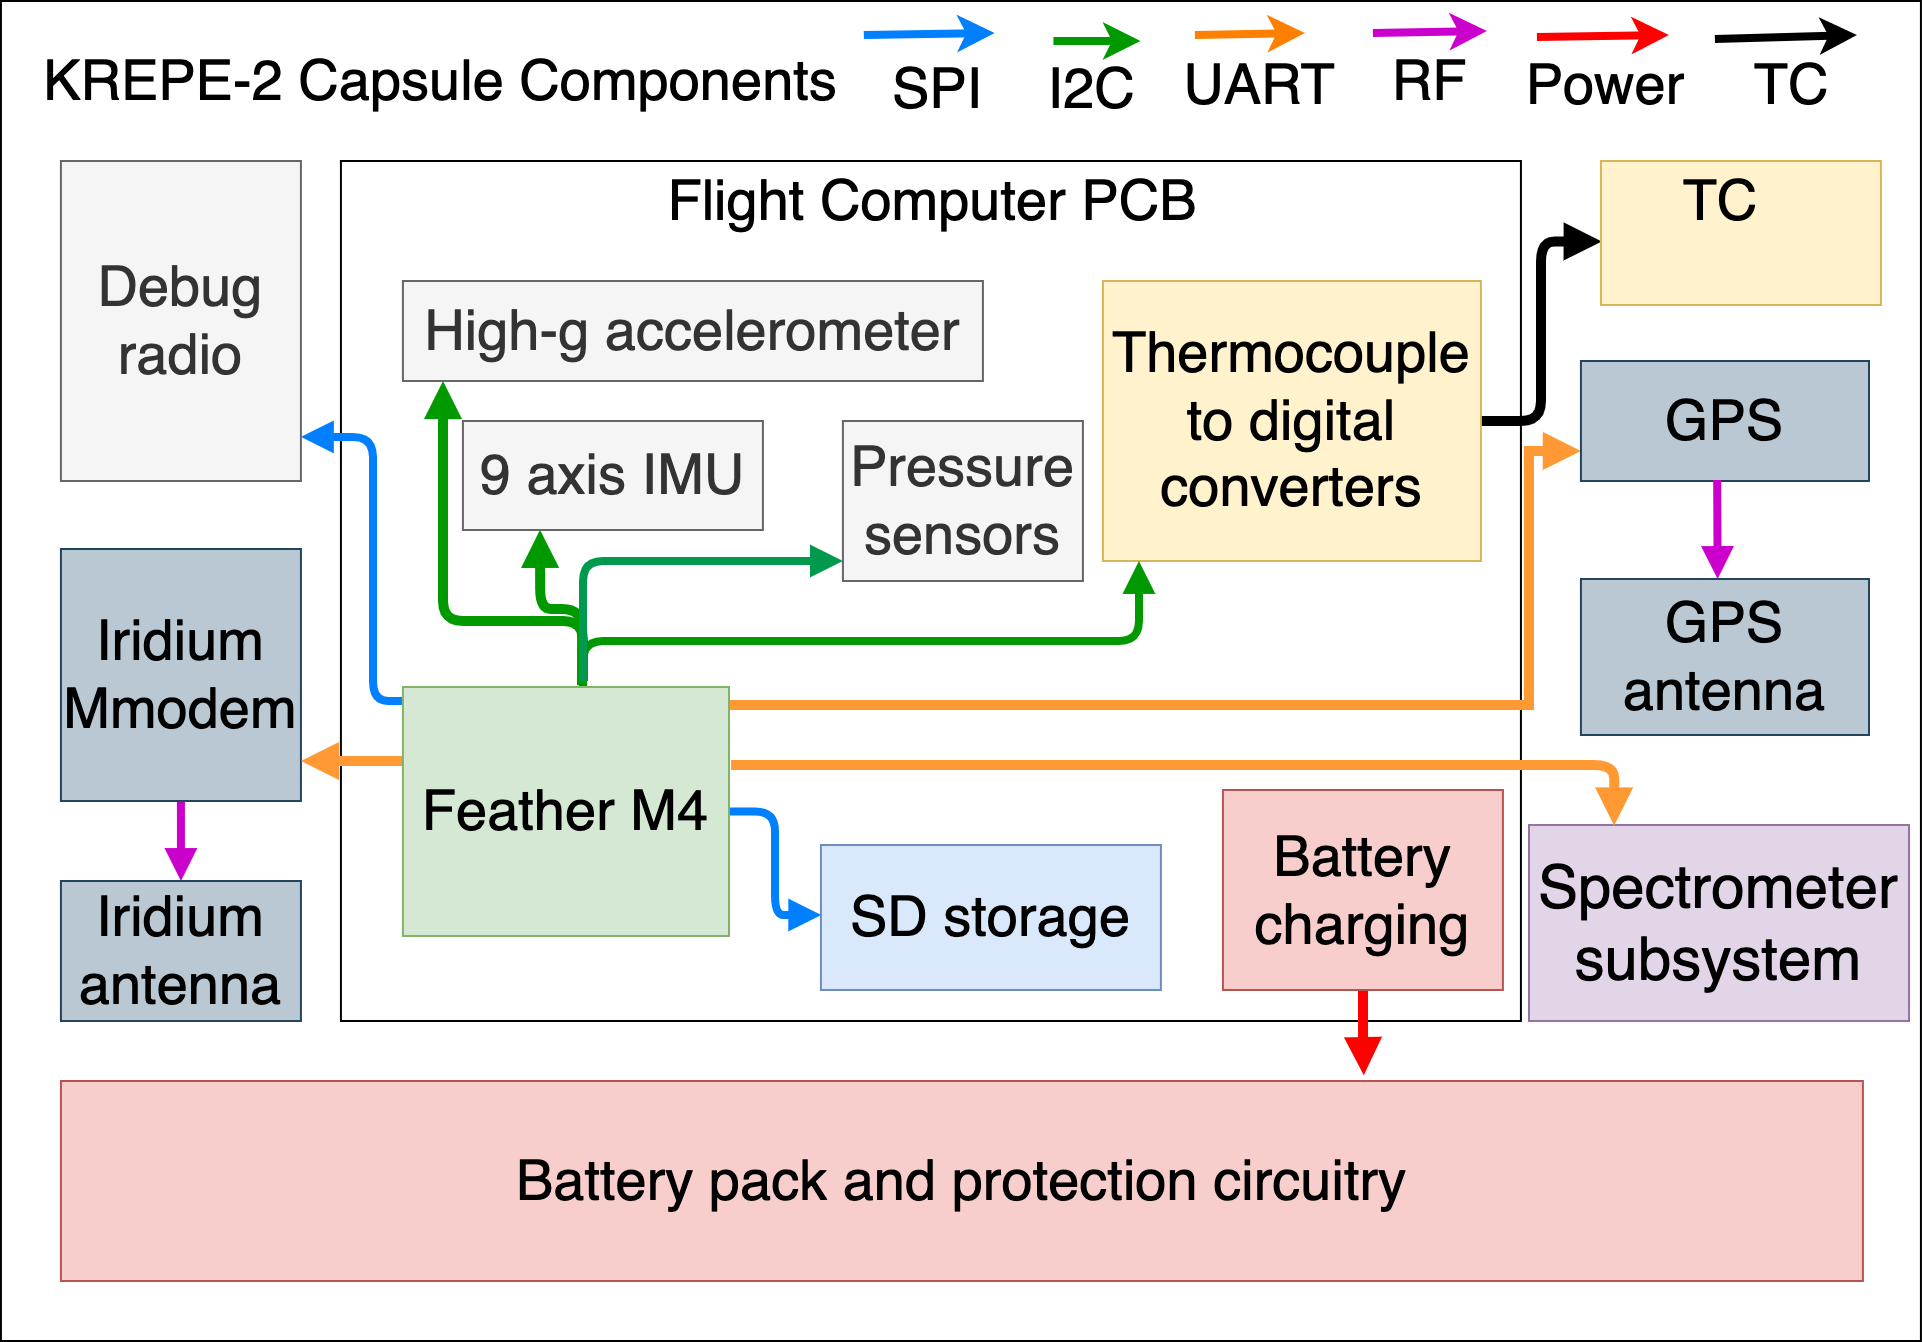
\includegraphics[width=12cm]{images/krepe2-avionics.png}
    \caption{Activation and battery protection schematic overview.}
    \label{fig:activation-circuitry}
\end{figure}



%There is an low power 915MHz ISM band debug communication link that is only used during testing on the ground and is physically disconnected from power before once handed over for final integration. The \texttt{ISM\_SW} header is meant to enable and disable the RFM69 debug radio. The center 3.3V pin of this header is connected to the normally closed labeled pin, a GPIO pin is pulled high (see Fig. \ref{tab:pins_radio}). When the normally closed pin is connected to the center pin, the RFM69 is enabled. 




\subsection{Secondary Activation}
\label{sec:secondary-activation}
Once primary activation is complete and the flight computer is in dormant mode, a digital input to the flight computer is configured as an interrupt to sense when the KREM separates from around the capsule. When this interrupt is triggered and the  register a temperature that is sufficient to have melted the polycarbonate bolts that hold the KREM together, secondary activation occurs. If the temperature is not sufficient, the flight computer re-enters dormant mode. No radio transmissions are attempted before secondary activation. 

%Thermocouples and the KREM interrupt sensing subsystem are polled to check for conditions sufficient for secondary activation. As KREPE re-enters the atmosphere, heating of the metal KREM will melt the plastic bolts that hold it together. This ambient temperature increase of the probe is sensed by the thermal measurement subsystem and is one criteria for secondary activation. The presence of KREM around the probe is detected by capacitive sensors, this is the secondary criteria for secondary activation. Once the thermal and capacitive sensing subsystems have detected the separation of the metal enclosure, the Iridium radio is powered on and packet transmission begins.  

%An activation redundancy processor (ARP) was added in Rev. 1.1 of the flight computer, if the flight computer needs to be tested without the ARP, there is a solder jumper on the bottom of the PCB (SJ1) that, when shorted together, bypasses the AND gate that controls Iridium radio activation, reducing the system to single activation.




%%%%%%%%%%%%%%%%%%%%%%%%%%%%%%%%%%%%%%%%%%%%%%%%%%%%%%%%%%%%%%%%%%%%%%%%%%%%%%%%%%%%%%%%%
%%%%%%%%%%%%%%%%%%%%%%%%%%%%%%%%%%%%%%%%%%%%%%%%%%%%%%%%%%%%%%%%%%%%%%%%%%%%%%%%%%%%%%%%%
%%%%%%%%%%%%%%%%%%%%%%%%%%%%%%%%%%%%%%%%%%%%%%%%%%%%%%%%%%%%%%%%%%%%%%%%%%%%%%%%%%%%%%%%%
%%%%%%%%%%%%%%%%%%%%%%%%%%%%%%%%%%%%%%%%%%%%%%%%%%%%%%%%%%%%%%%%%%%%%%%%%%%%%%%%%%%%%%%%%
%%%%%%%%%%%%%%%%%%%%%%%%%%%%%%%%%%%%%%%%%%%%%%%%%%%%%%%%%%%%%%%%%%%%%%%%%%%%%%%%%%%%%%%%%
%%%%%%%%%%%%%%%%%%%%%%%%%%%%%%%%%%%%%%%%%%%%%%%%%%%%%%%%%%%%%%%%%%%%%%%%%%%%%%%%%%%%%%%%%
%%%%%%%%%%%%%%%%%%%%%%%%%%%%%%%%%%%%%%%%%%%%%%%%%%%%%%%%%%%%%%%%%%%%%%%%%%%%%%%%%%%%%%%%%
%%%%%%%%%%%%%%%%%%%%%%%%%%%%%%%%%%%%%%%%%%%%%%%%%%%%%%%%%%%%%%%%%%%%%%%%%%%%%%%%%%%%%%%%%
\section{Subsystems}
\label{sec:subsystems}

\subsection{Radio Communications}

KREPE has two radios, a debug radio used for ground work and an Iridium satellite modem used both on the ground and during the mission. The following subsections explain the conditions necessary for enabling the satellite modem during the mission and also restate that the debug radio is physically disabled prior to final integration and is never powered on or used during the actual mission.

\subsubsection{Radio Power Control}
\label{sec:radio-power-control}
There are two inhibits to powering on the iridium, as denoted in Table~\ref{tab:radio-inhibits}. The separation of the KREM must be detected and the temperature of the capsule must be determined to be above the activation threshold temperature, $T_a$.
%Two indeAn AND gate controls the power to the solid state relay controlling power to the Iridium radio. The secondary processor is connected to the other input of this AND gate to make sure that erroneous action on behalf the Teensy (or secondary safety processor) is not able to solely activate the radio. In addition to the thermocouple measurements, another inhibit to powering on the Iridium radio is the detection of KREM separation, performed by capacitive sensing. Table \ref{tab:radio-inhibits} summarizes the inhibits to radio activation.


\begin{table}[H]
	\caption{Inhibits to Ididium radio activation.}
	\label{tab:radio-inhibits}
	\centering
	\begin{tabular}{l|l|l}
		Sensor & Monitored by     &  Description  \\
		\hline
		
		Thermocouples & Teensy  & Thermocouple temperature reported by Teensy\\
		%Thermocouples & ARP		& Thermocouple temperature reported by secondary ARP \\
		KREM Interrupt	 & Teensy  & KREM presence detected by Teensy
	\end{tabular}
	
\end{table}



\subsubsection{Iriduim Radio}
We are using the A3LA-RS type modem seen on the NAL Research site~\footnote{ \url{http://www.nalresearch.com/IridiumHardware.html}}. The RF specifications, taken from the module's datasheet are shown in Fig. \ref{fig:iridium-rf-specs}.

\begin{figure}[H]
    \centering
    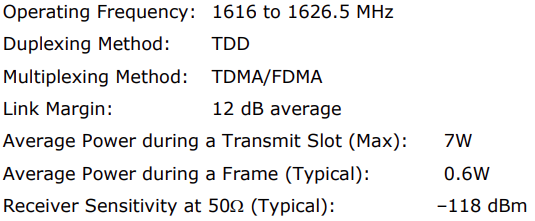
\includegraphics[width=0.5\textwidth]{images/iridium-rf-specs.png}
    \caption{RF specifications of the AL3A-RS Iridium modem.}
    \label{fig:iridium-rf-specs}
\end{figure}

\paragraph{Iridium Serial Interface}

A 3.3V TTL to RS232 adapter is needed to interface with the AL3A-RS. As an improvement over KREPE-1, this chip is integrated onto the flight computer for more compact design and higher convenience. The serial converter uses a  MAX3232E RS-232 line driver and receiver~\footnote{\url{https://www.ti.com/product/MAX3232E}}.



\subsubsection{Debug Radio}
The KREPE flight computer features a secondary debug radio used for ground testing that is not enabled for the real mission.  Maximum output power according to the radio datasheet \footnote{\url{https://cdn.sparkfun.com/datasheets/Wireless/General/RFM69HCW-V1.1.pdf}} is 100mW.
\begin{table}[H]
	\centering
	\caption{Radio module interface signals.}
	\label{tab:pins_radio}
	\begin{tabular}{l|l|l|l}
		Feather M4 Pin & Net Name  & Description   & Teensy Configuration \\
		\hline 
		28 & RADIO\_RESET  &  Pull low to enable RFM69   & \texttt{OUTPUT} 
		%29 & INT\_ISM    &  GPIO0 interrupt from RFM69 & \texttt{INPUT} \\
		%33 & RADIO\_OFF\_SIG & Pulled high when the RFM69 is disabled & \texttt{INPUT} \\
	\end{tabular}
\end{table}
The datasheet for this antenna can be found at  \url{https://cdn.taoglas.com/datasheets/FXP290.07.0100A.pdf}. 
  


\subsection{Thermal Measurement}
The thermal measurement subsystem is used to take readings from up to six thermocouples (TCs) embedded within the TPS surrounding each capsule. 

\subsubsection{Thermocouple Connections}

The thermocouple to digital conversion system on KREPE-2 uses 6 MCP-9600 TC to digital converters linked via I2C bus. This is an improvement over the multiplexed converter setup used in the first KREPE mission. A low pass filter is included between the TC connector points and each MCP-9600 to help suppress spurious measurements.
%
\begin{figure}[H]
    \centering
    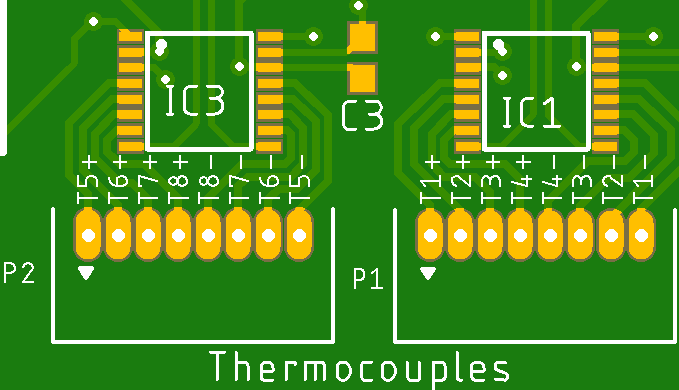
\includegraphics[width=0.5\textwidth]{images/krepe-thermocouples.png}
    \caption{NEED TO UPDATE THIS, SHOE THREAD iNSERTS!!!Thermocouple connection wiring with resepect to the analog mux chips IC3 (MUX2) and IC1 (MUX1).}
    \label{fig:tc-conn}
\end{figure}


%%%%%%%%%%%%%%%%%%%%%%%%%%%%%%%%%%%%%%%%%%%%%%%%
\subsection{FADS Pressure Measurement}

%%%%%%%%%%%%%%%%%%%%%%%%%%%%%%%%%%%%%%%%%%%%%%%%%%%%%%%%%%%%%
\subsection{Visual Status Indicators}
There are individual LEDs on the POL switches connected to each serial port header, in addition to an indicator on the external 3v3 regulator. In addition to these indicators, the Feather M4 board also has an RGB led that is used to indicate program state


The KREPE flight computer features several light emitting diodes (LEDs) to provide visual feedback during ground testing. Pin mappings and intended information denoted by each LED is shown in Table \ref{tab:pins_leds}.
\begin{table}[H]
	\centering
	\caption{Debug LED Connections.}
	\label{tab:pins_leds}
	\begin{tabular}{l|l|l}
		Teensy Pin & Net Name     & Teensy Configuration \\
		\hline 
		3 & LED1 - IRIDIUM ON        &   \texttt{OUTPUT}\\
		4 & LED2 - IRIDIUM SIGNAL OK       &   \texttt{OUTPUT}\\
		5 & LED3 - IRIDIUM RADIO TRANSMITTING       &   \texttt{OUTPUT}\\
		6 & LED4 - ISM RADIO TRANSMITTING       &   \texttt{OUTPUT}\\
		7 & LED5 - GENERAL ACTIVITY       &   \texttt{OUTPUT}
	\end{tabular}
\end{table}


%%%%%%%%%%%%%%%%%%%%%%%%%%%%%%%%%%%%%%%%%%%%%%%%%%%%%%%%%%%%%
\subsection{Auxillary Sensors}
The KREPE flight computer features several auxillary sensors that will be used to better characterize reentry. Measurements from an ADXL377 3-axis $\pm$200g accelerometer, ICM-20948 9-axis IMU, and DSP310 barometric pressure sensor are collected after secondary activation. Measurements from these auxiliary sensors are not used for activation.

\begin{table}[H]
    \centering
    \caption{Pins connecting to the ADXL377 and ICM-20948.}
    \label{tab:pins_motionsensor}
    \begin{tabular}{c|c|c|r}
    Teensy Pin & Net Name  & Description   & Teensy Configuration \\
    \hline 
    36 A17 & XOUT & Analog out from accel (x axis) & \texttt{INPUT} \\
    37 A18 & YOUT & Analog out from accel (y axis) & \texttt{INPUT} \\
    38 A19 & ZOUT & Analog out from accel (z axis) & \texttt{INPUT} \\
    35 & INT & Interrupt from ICM-20948 & \texttt{INPUT} \\
    34 & FSYNC & Synchronization signal to ICM-20948 & \texttt{OUTPUT} 
    \end{tabular}
\end{table}

%\paragraph{Barometric Pressure Sensor}
%Version 1.1 of the flight computer features an Infineon DSP310 barometric pressure and temperature sensor connected to the SPI bus with active low chip select on pin 8 of the Teensy. This sensor is not used for activation detection. 



%%%%%%%%%%%%%%%%%%%%%%%%%%%%%%%%%%%%%%%%%%%%%%%%%%%%%%%%%%%%%%%55
\subsection{Power and Batteries}
Batteries are provided by JSC and rated at 3200mAh. System power is provided by two of these cells tabbed in parallel (tabbing performed and documented by JSC). Battery classification, product, and model number can be seen in Fig. \ref{fig:bat-spec} (taken from battery specification sheet).

\begin{figure}[h!]
	\centering
	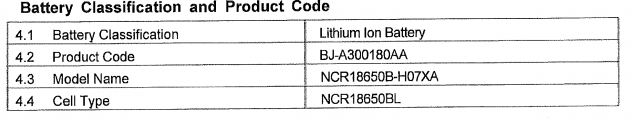
\includegraphics[width=12cm]{images/battery-spec.png}
	\label{fig:bat-spec}
	\caption{Sanyo battery specifications from the datasheet.}
\end{figure}

Charge current is limited to to 450 milliamps (mA), a charge rate of $C/12$ with the two (2) 3200 milliamp-hour (mAh) system  Battery Charge power can be delivered via Teensy USB or the \texttt{CHARGE} header. Charging input voltage is expected to be 5 volts. Charge voltage to the batteries is regulated to 4.2 volts by the charge management IC, an MCP73831\footnote{ (\url{https://www.microchip.com/wwwproducts/en/MCP73831})}, with status connections to the Teensy as shown in Table \ref{tab:pins-battery}. 

charging when not installed vs charging when installed.

Charging is only performed on the ground and there is no provision for charging in flight. Schematics and electrical connections are shown in Fig. \ref{fig:page1-3} in Appendix \ref{appa}.

\subsubsection{Battery Status Interface}
\begin{table}[H]
    \centering
    \caption{Pins to monitor battery voltage and charging status.}
	\label{tab:pins-battery}
    \begin{tabular}{c|c|c|r}
    Teensy Pin & Net Name  & Description   & Teensy Configuration \\
    \hline 
    14 & BAT\_STAT & LiPo charge state & \texttt{OUTPUT} \\
    22 A8 & BAT\_SENSE    &  Halved battery voltage for monitoring &   \texttt{INPUT} 
    \end{tabular}
\end{table}

\subsubsection{Battery Protection}
Protection circuitry is implemented on the flight board to support 2P1S LiIon packs for system power. We are using a DW01-P Voltage and Current Protection IC \footnote{\url{https://cdn.sparkfun.com/assets/learn_tutorials/2/5/1/DW01-P_DataSheet_V10.pdf}}.


\begin{figure}[H]
	\centering
	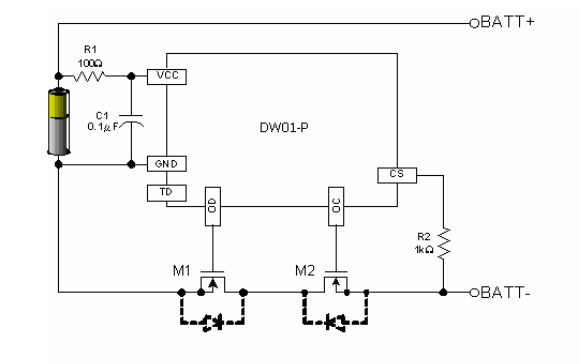
\includegraphics[width=0.6\textwidth]{images/dw108.png}
	\caption{Battery protection circuitry.}
	\label{fig:bat-protec}
\end{figure}



Protection circuitry as implemented on the KREPE flight computer PCB is shown in Fig. \ref{fig:bat-protec}. Our two batteries are in parallel where the battery image is shown in Fig. \ref{fig:bat-protec}, and BATT+ and BATT- face system power i.e. to the flight computer. This protection circuitry is upstream of the primary activation switch. The battery protection PCB can be seen in Fig. \ref{fig:bat-protect}.


\begin{figure}[H]
	\centering
	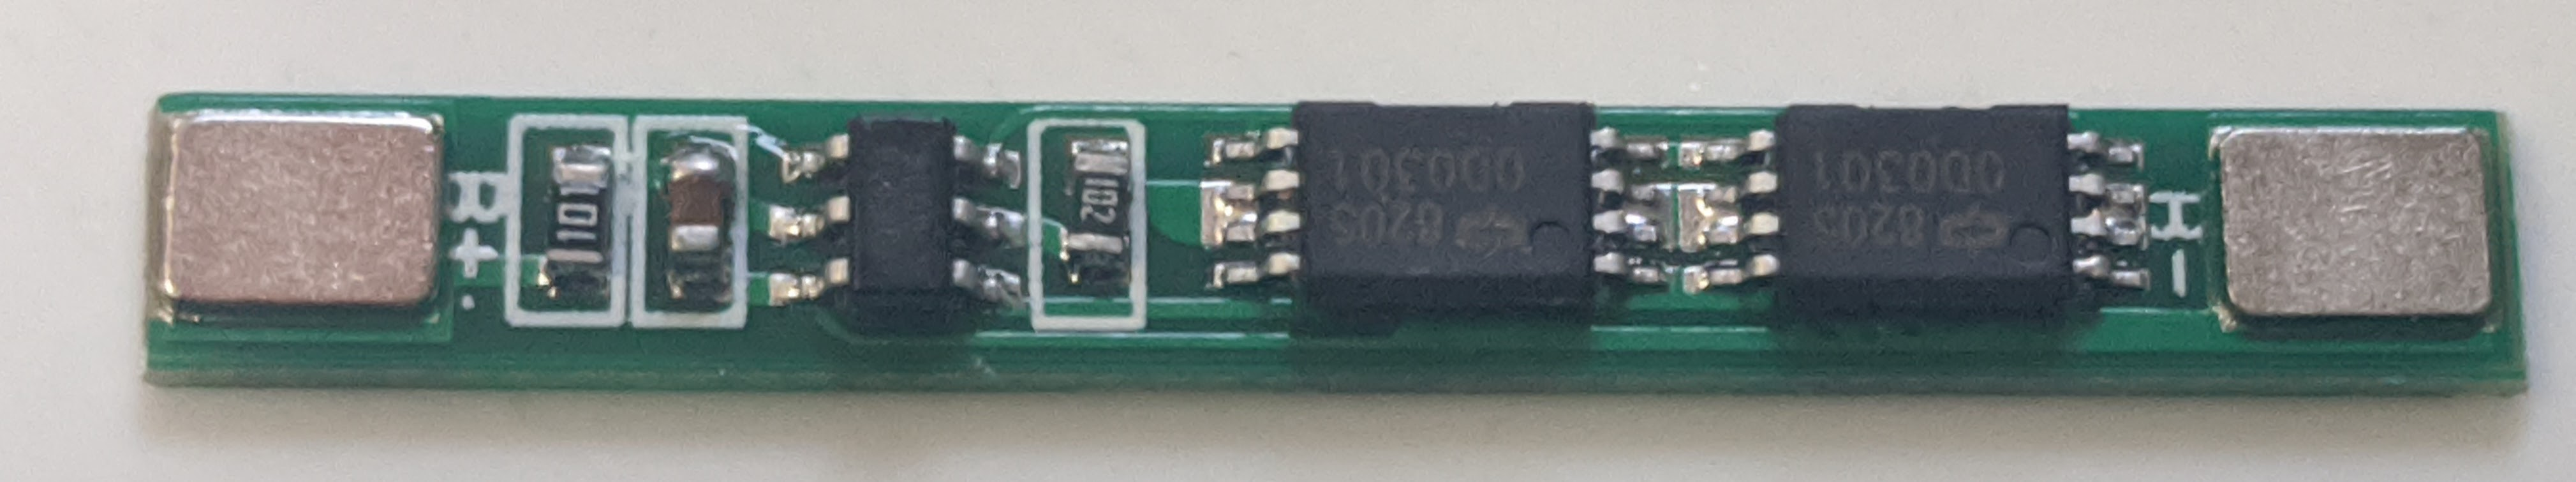
\includegraphics[width=0.5\textwidth]{images/new_batt_prot.png}
	\caption{Battery protection PCB.}
	\label{fig:bat-protect}
\end{figure}


\paragraph{Over-current protection}
The battery protection PCB can be seen preventing over current draw in Fig. \ref{fig:over-current}. After 6 milliseconds, the battery cells are disconnected from the output and current draw goes zero.


\begin{figure}[H]
	\centering
	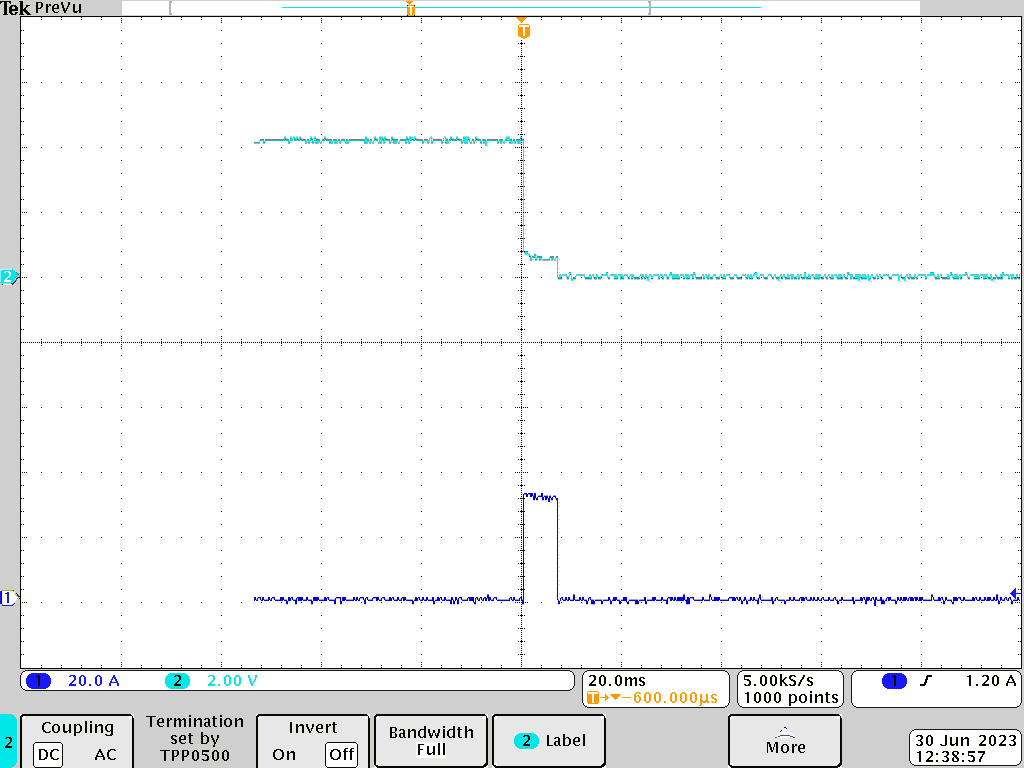
\includegraphics[width=0.9\textwidth]{images/over-current.png}
	\caption{The battery protection circuity disconnecting the cells after 6ms of over current condition. Blue: current. Purple: pack voltage.}
	\label{fig:over-current}
\end{figure}




%%%%%%%%%%%%%%%%%%%%%%%%%%%%%%%%%%%%%%%%%%%%%%%%%%%%%%%%%%%%%%%%%%%%%%%%%%%%%%%%%%%
%%%%%%%%%%%%%%%%%%%%%%%%%%%%%%%%%%%%%%%%%%%%%%%%%%%%%%%%%%%%%%%%%%%%%%%%%%%%%%%%%%%
%%%%%%%%%%%%%%%%%%%%%%%%%%%%%%%%  APPENDIX
%%%%%%%%%%%%%%%%%%%%%%%%%%%%%%%%%%%%%%%%%%%%%%%%%%%%%%%%%%%%%%%%%%%%%%%%%%%%%%%%%%%
%%%%%%%%%%%%%%%%%%%%%%%%%%%%%%%%%%%%%%%%%%%%%%%%%%%%%%%%%%%%%%%%%%%%%%%%%%%%%%%%%%%
\appendix


\section{Schematics}
\label{appa}

\begin{figure}[H]
    \centering
    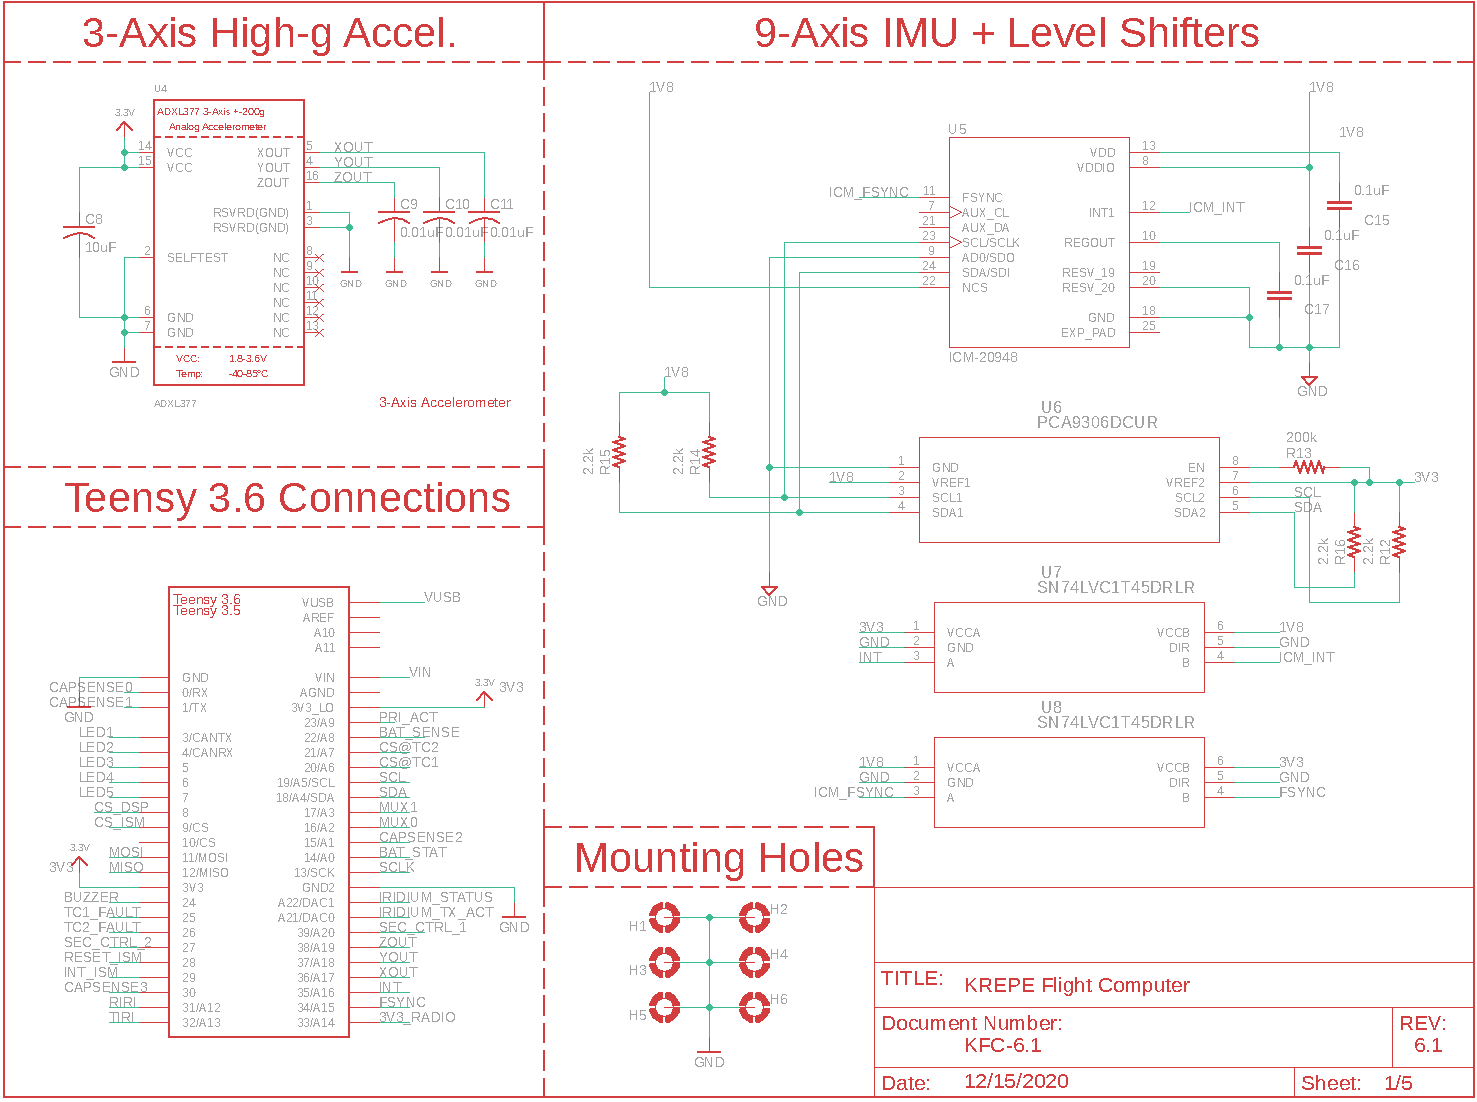
\includegraphics[width=\textwidth]{images/page1.png}
    \caption{Page one of schematics.}
    \label{fig:page1-2}
\end{figure}

\begin{figure}[H]
    \centering
    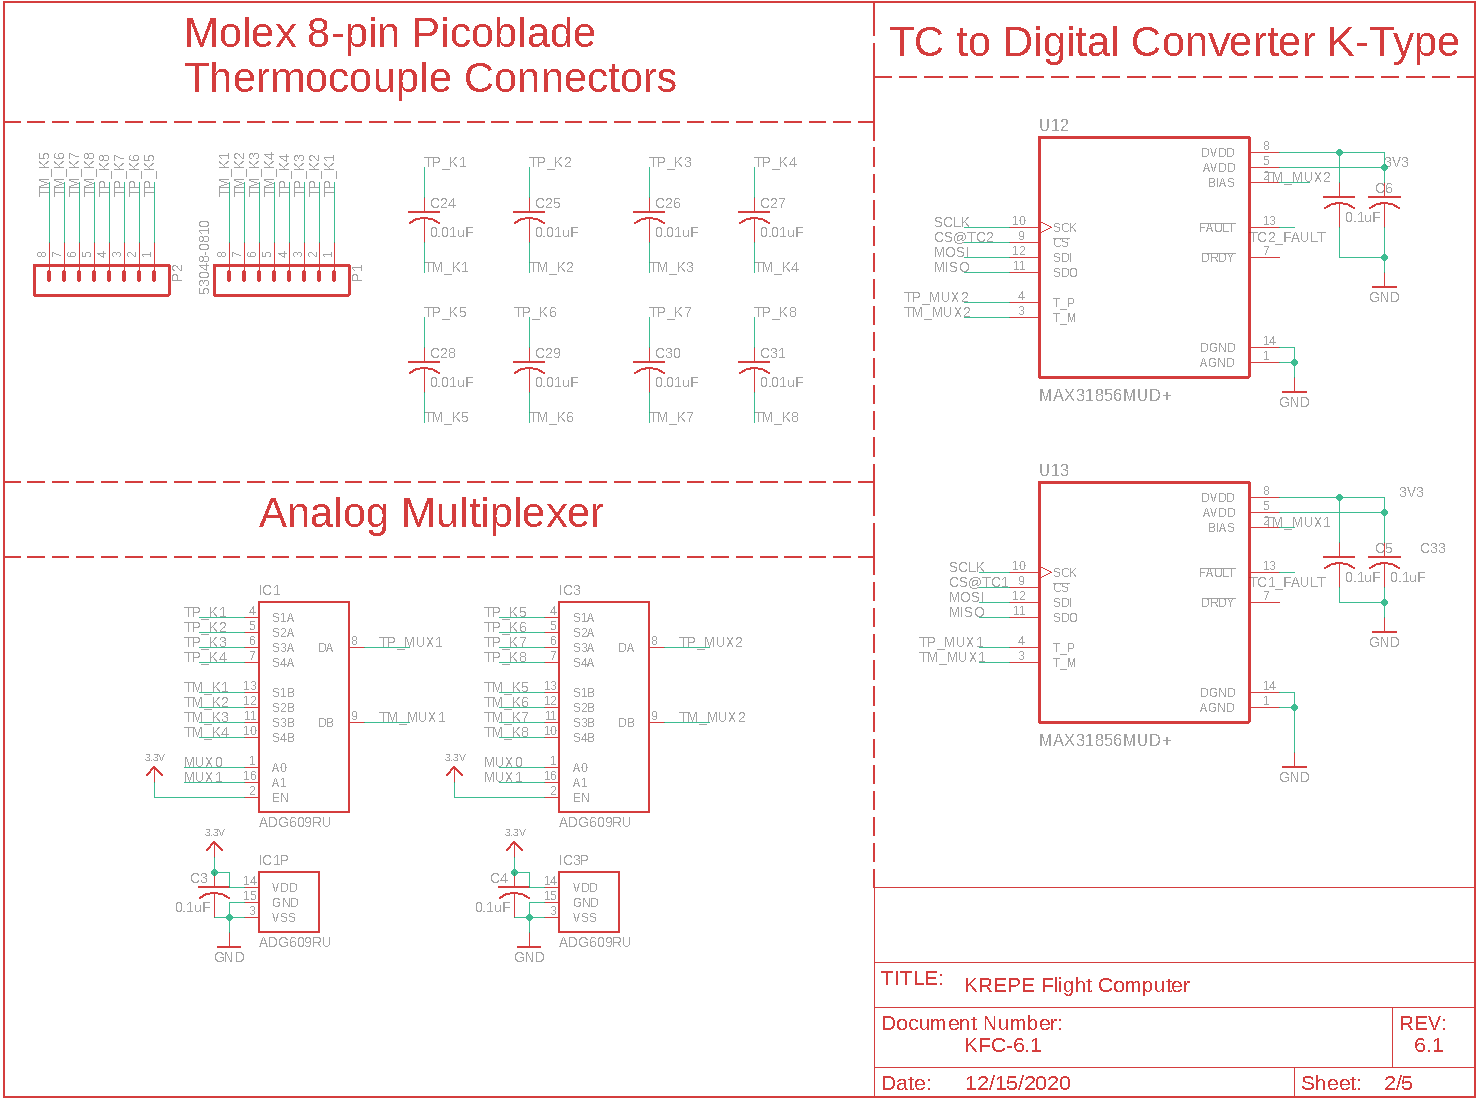
\includegraphics[width=\textwidth]{images/page2.png}
    \caption{Page two of schematics.}
    \label{fig:page1_1}
\end{figure}

\begin{figure}[H]
    \centering
    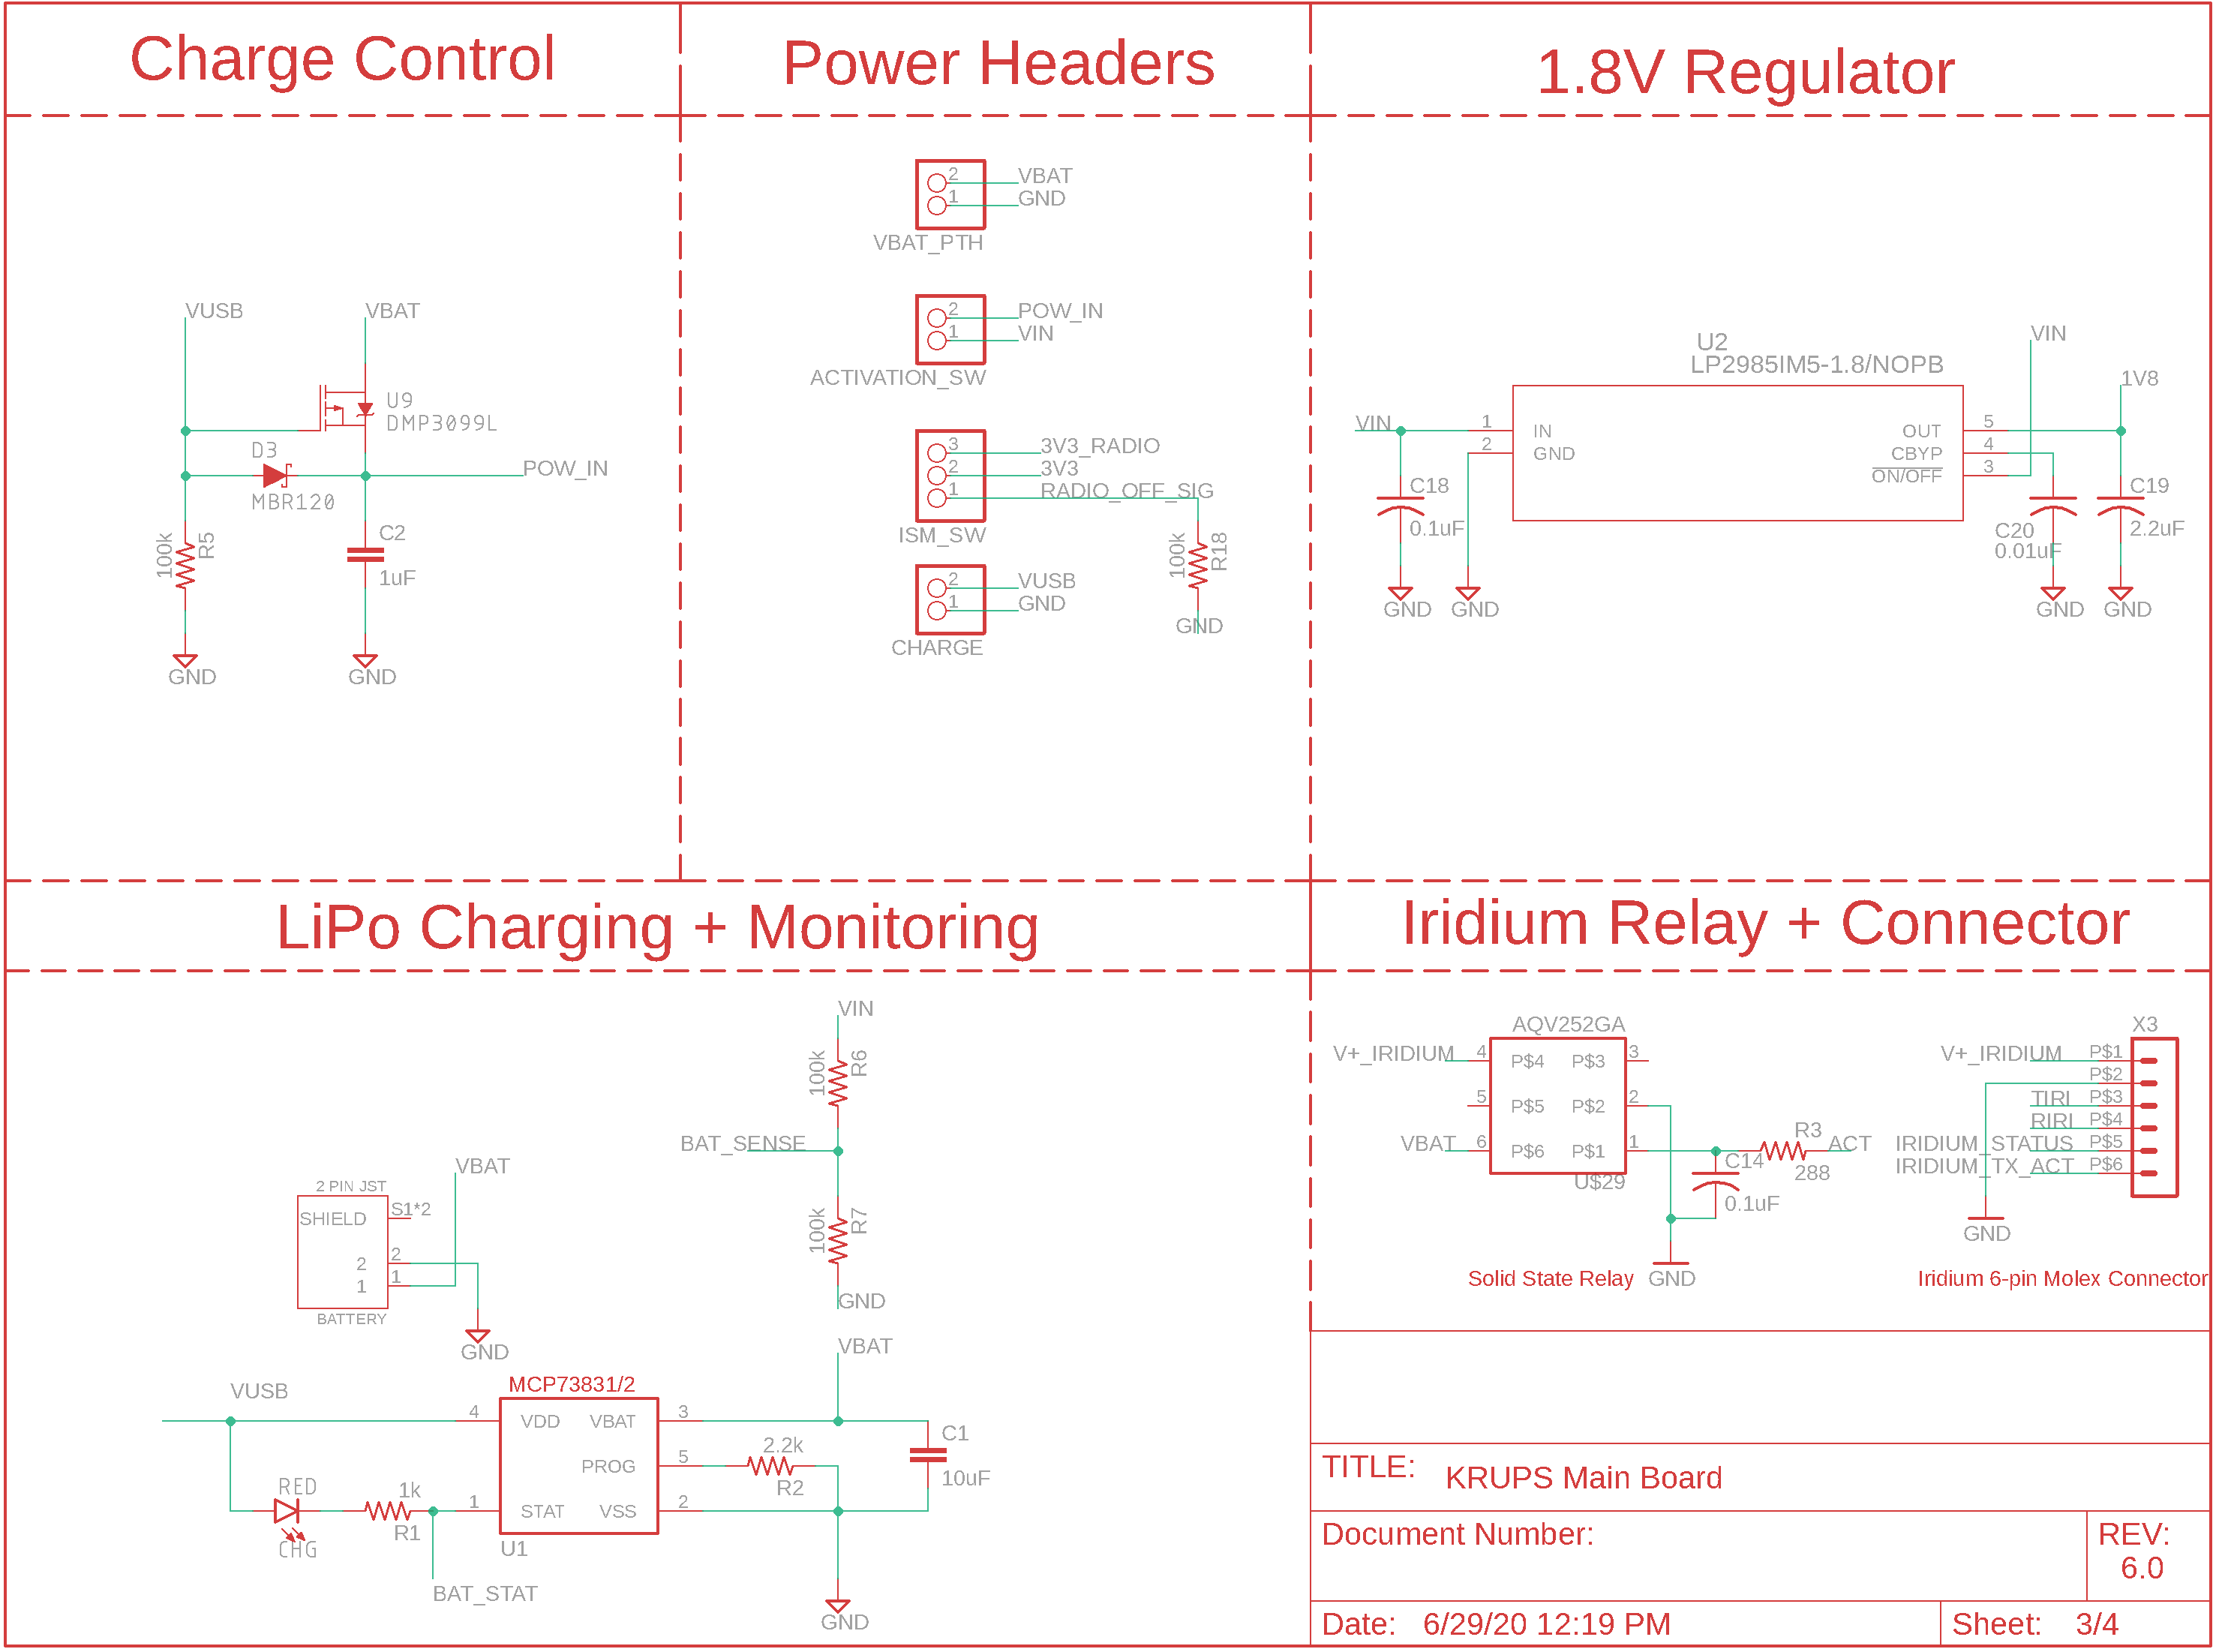
\includegraphics[width=\textwidth]{images/page3.png}
    \caption{Page three of schematics.}
    \label{fig:page1-3}
\end{figure}

\begin{figure}[H]
    \centering
    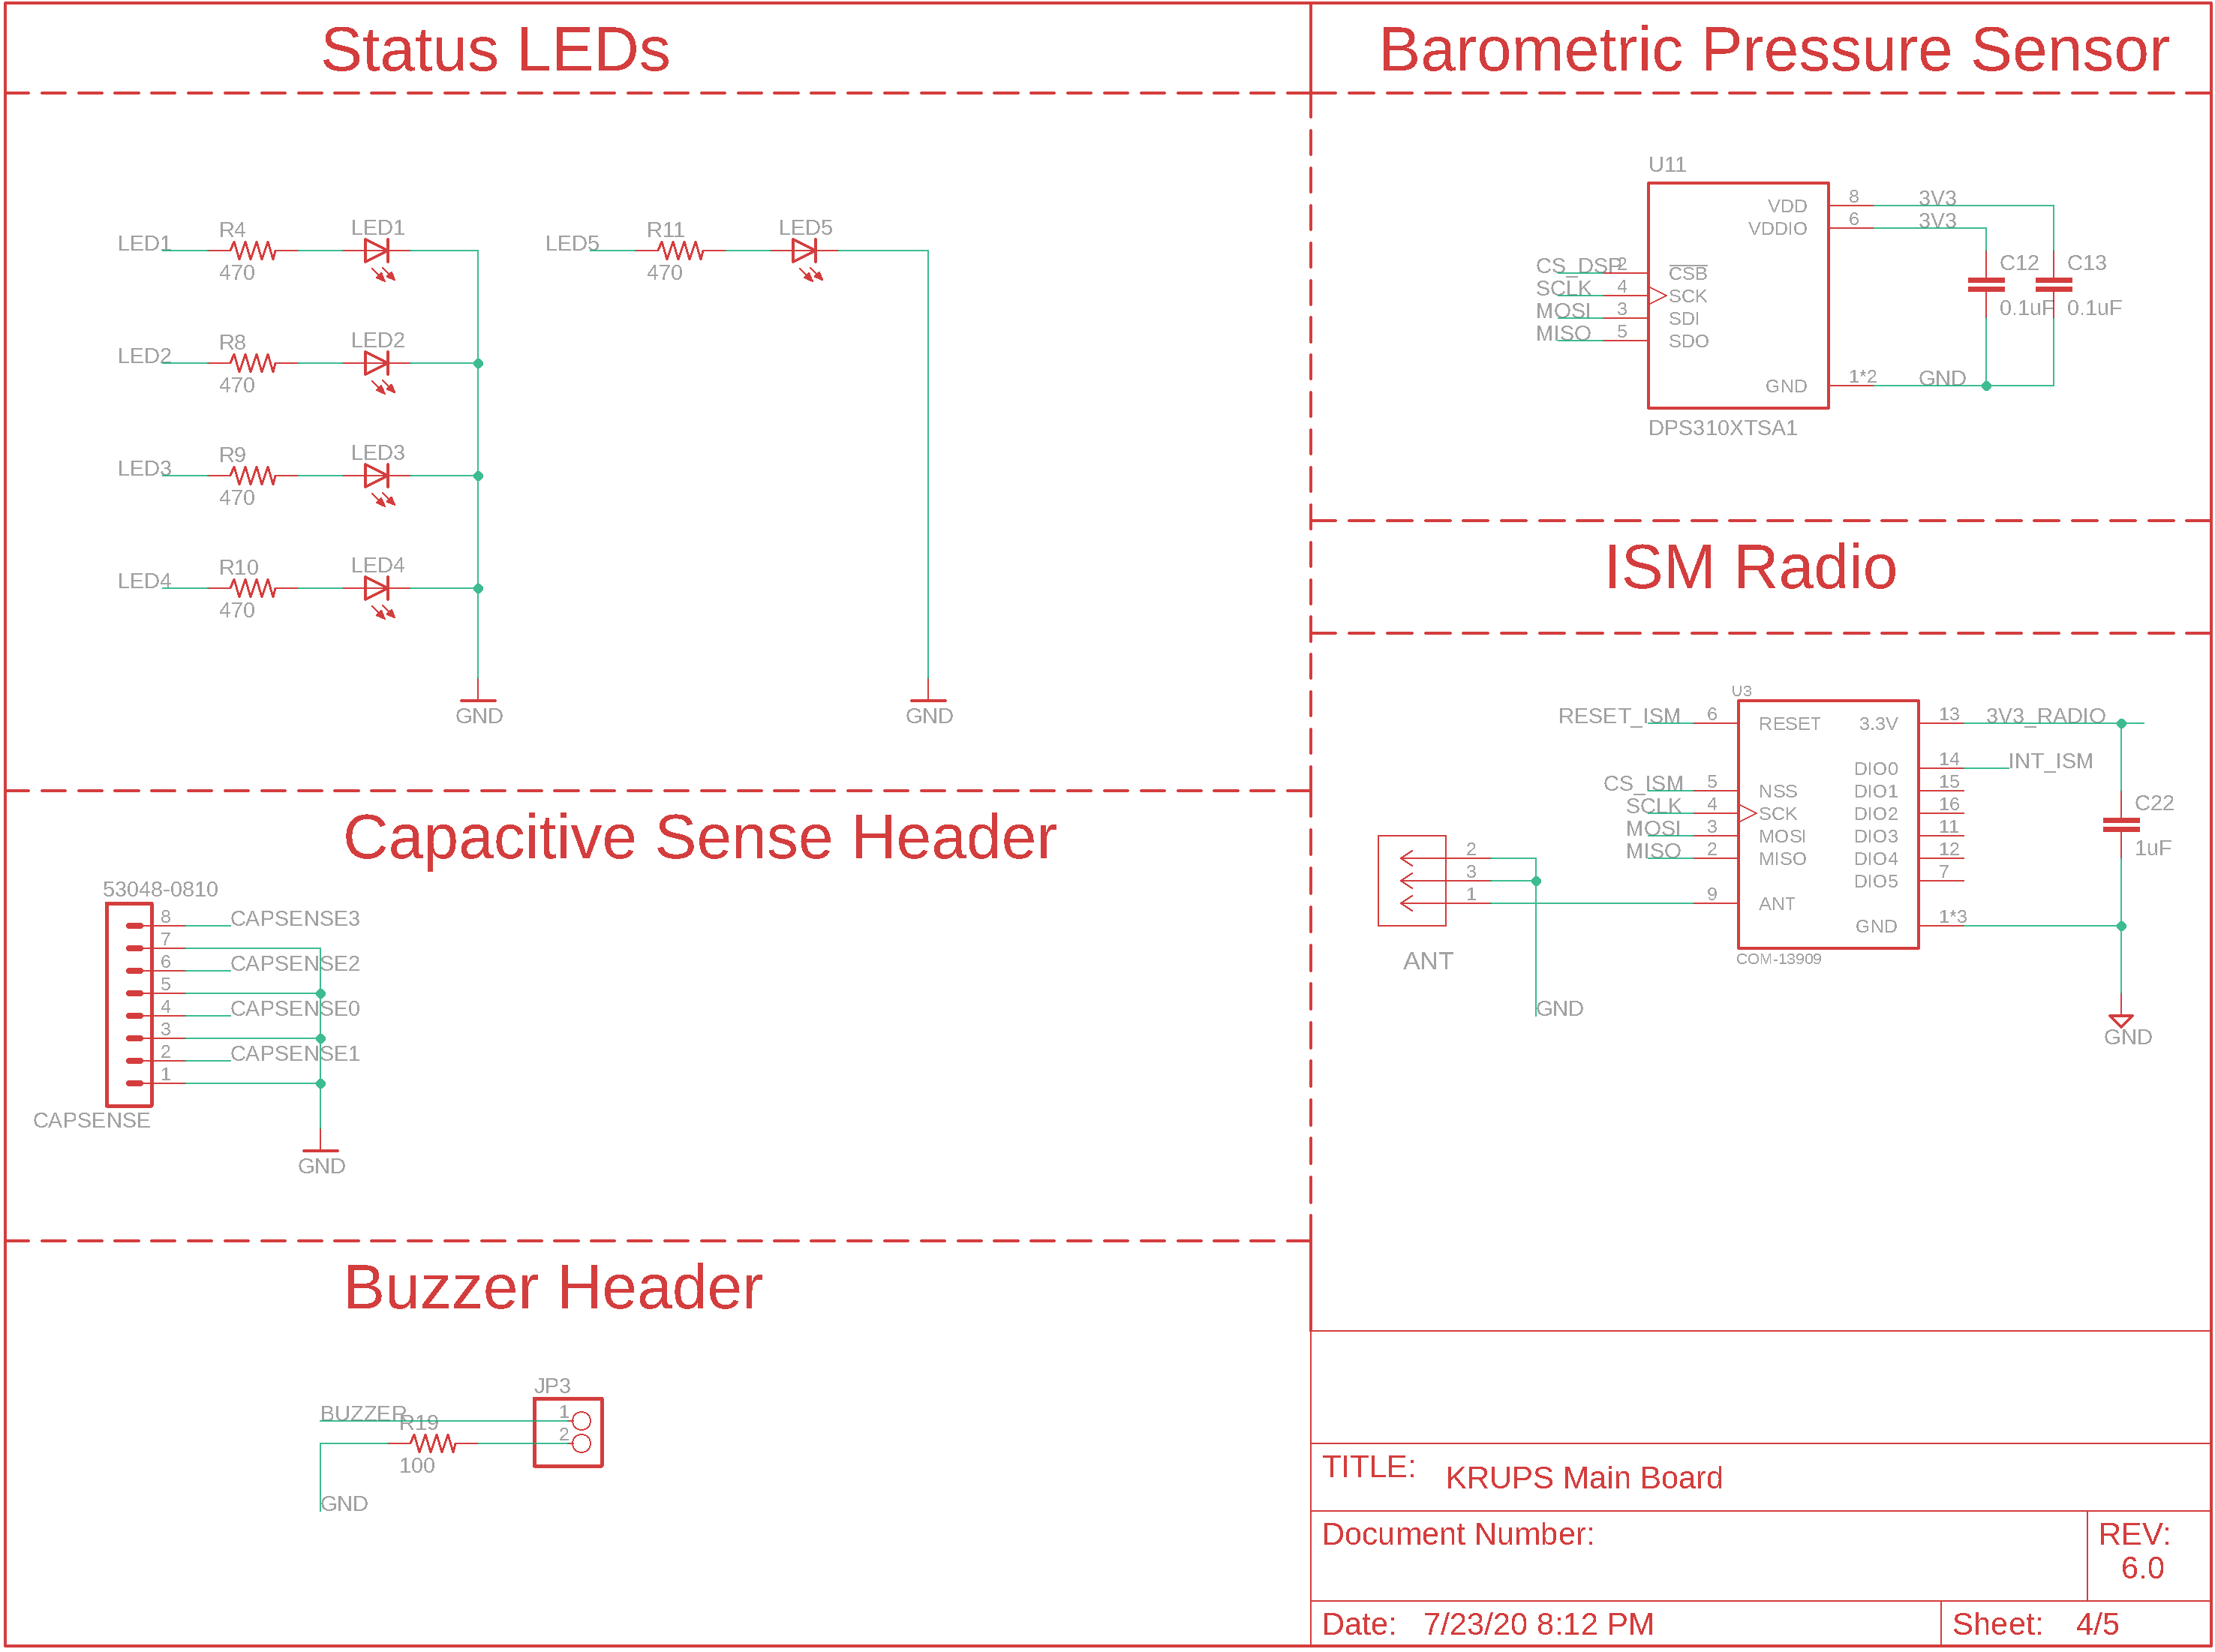
\includegraphics[width=\textwidth]{images/page4.png}
    \caption{Page four of schematics.}
    \label{fig:page1-4}
\end{figure}


%\begin{figure}[H]
%    \centering
%    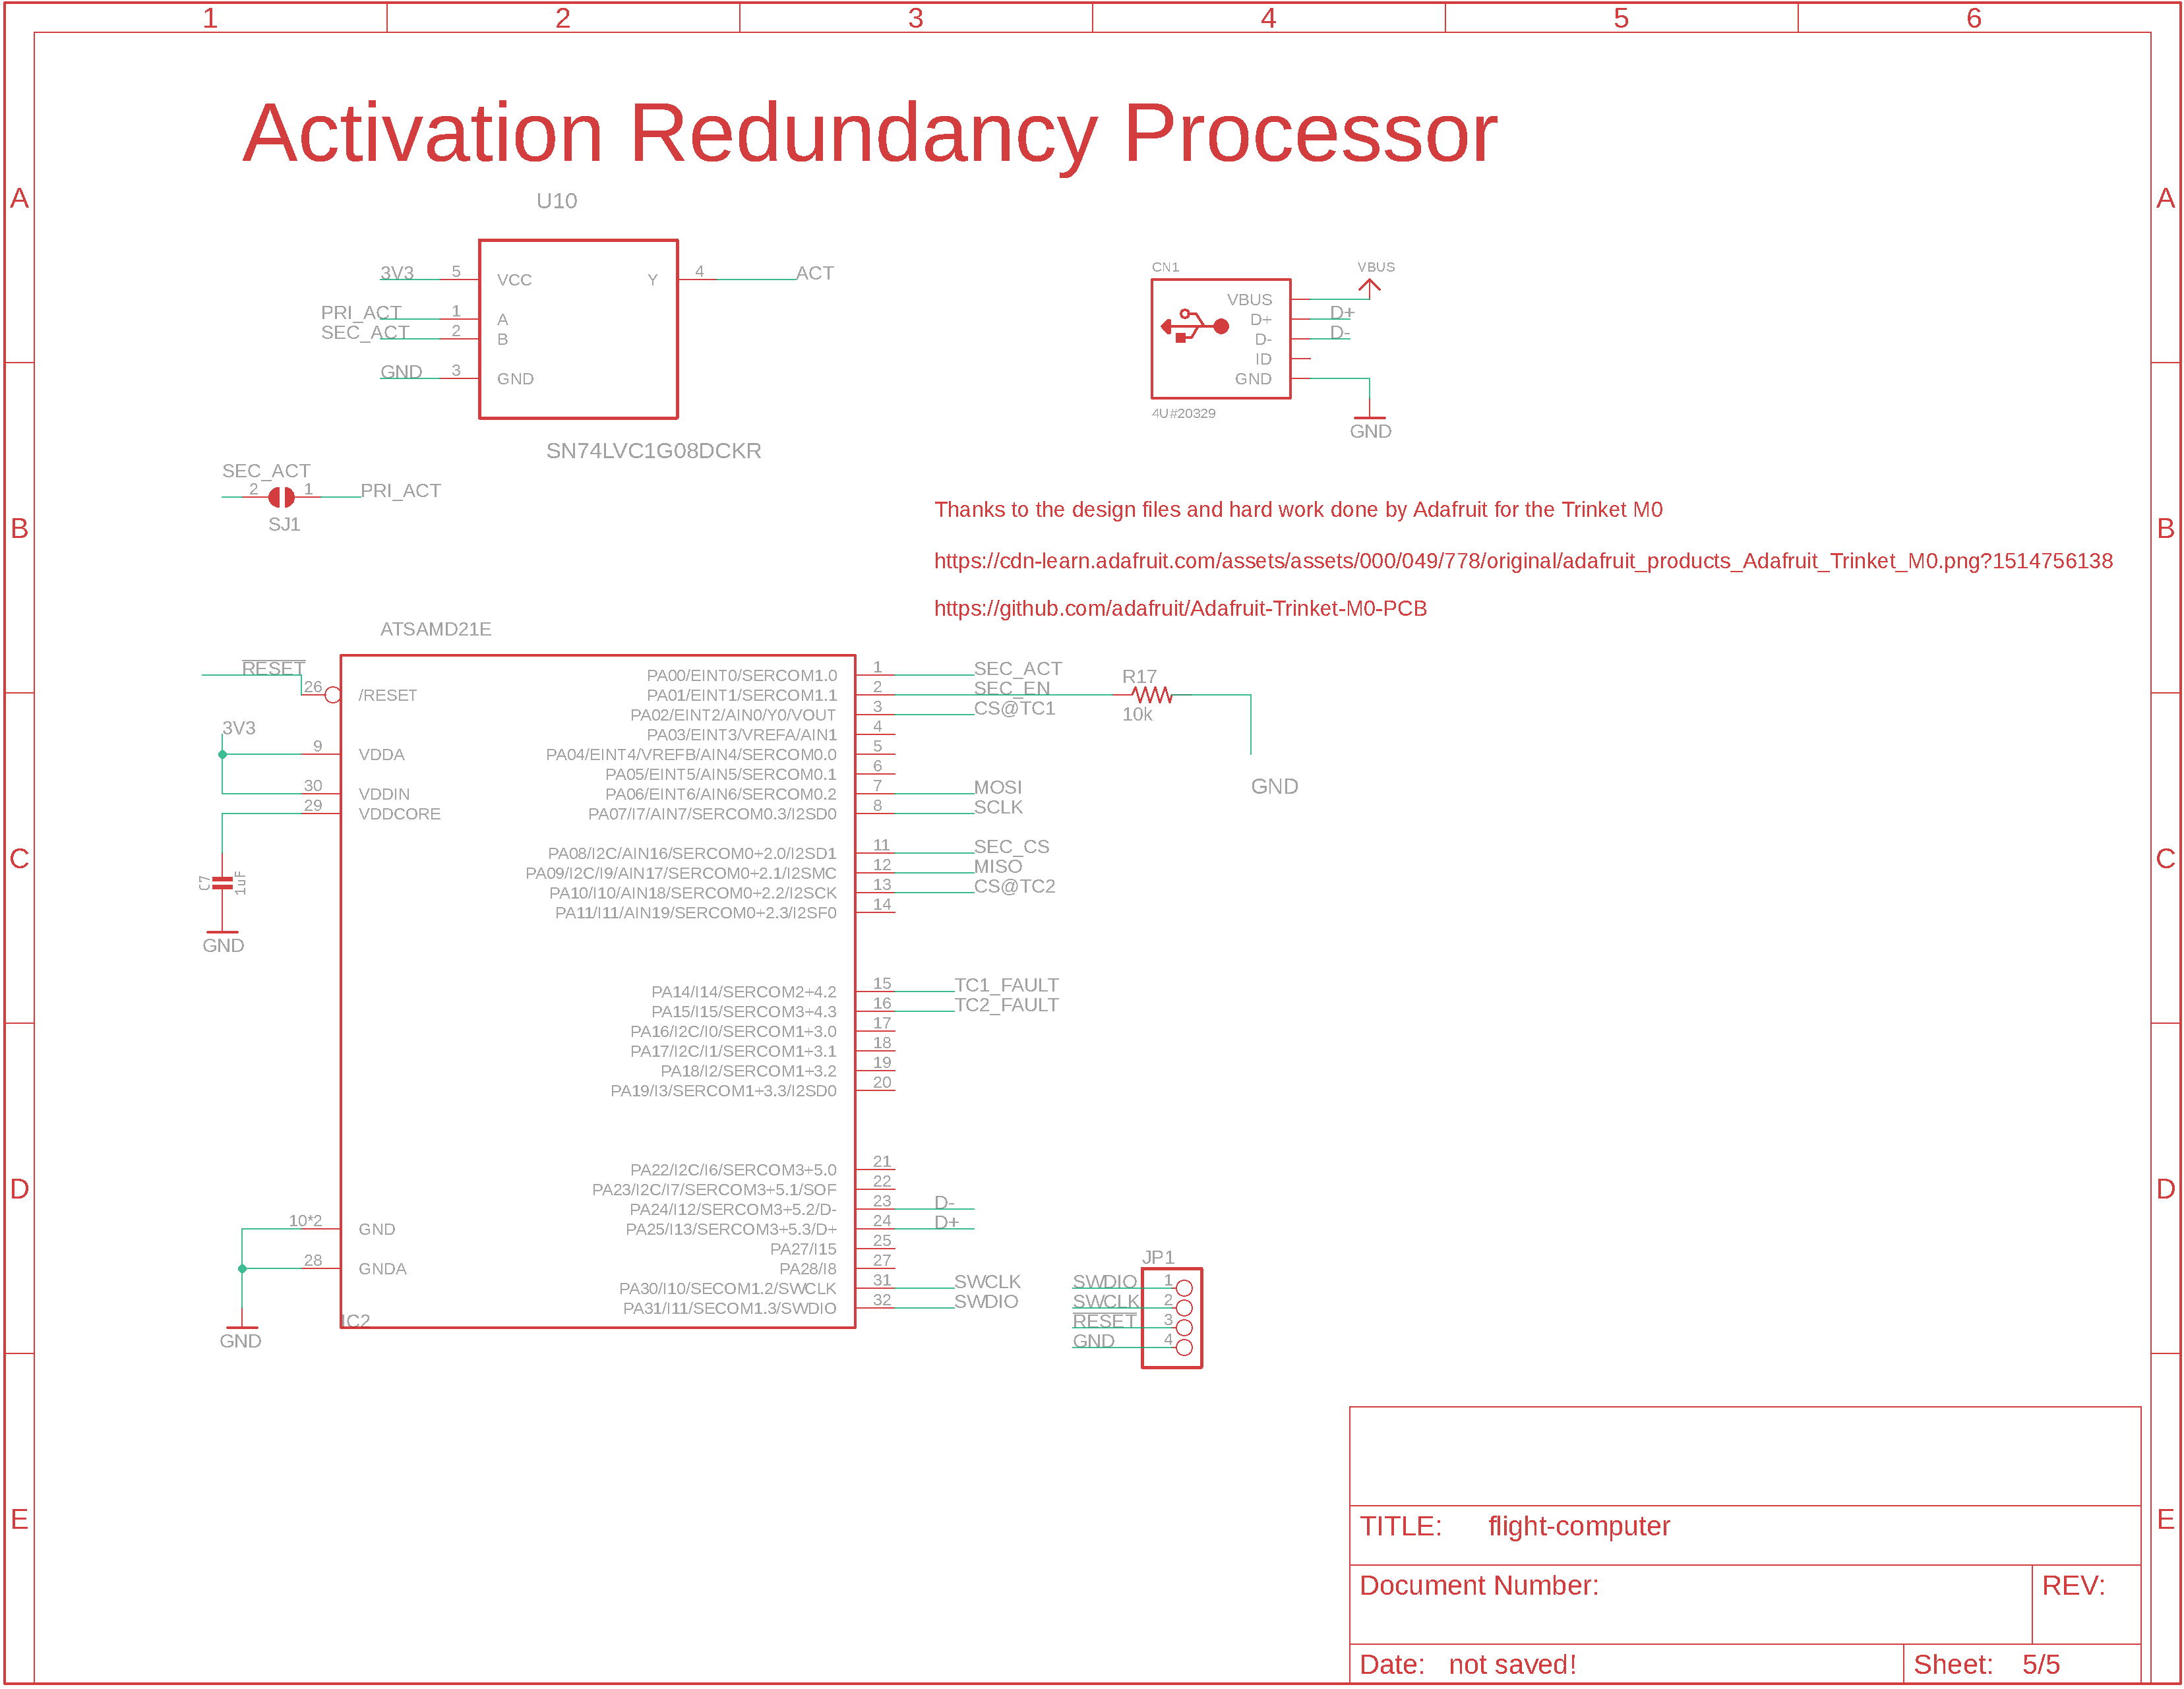
\includegraphics[width=\textwidth]{images/page5.png}
%    \caption{Page five of schematics.}
%    \label{fig:page1-5}
%\end{figure}

\section{Board Renderings}
\begin{figure}[H]
	\centering
	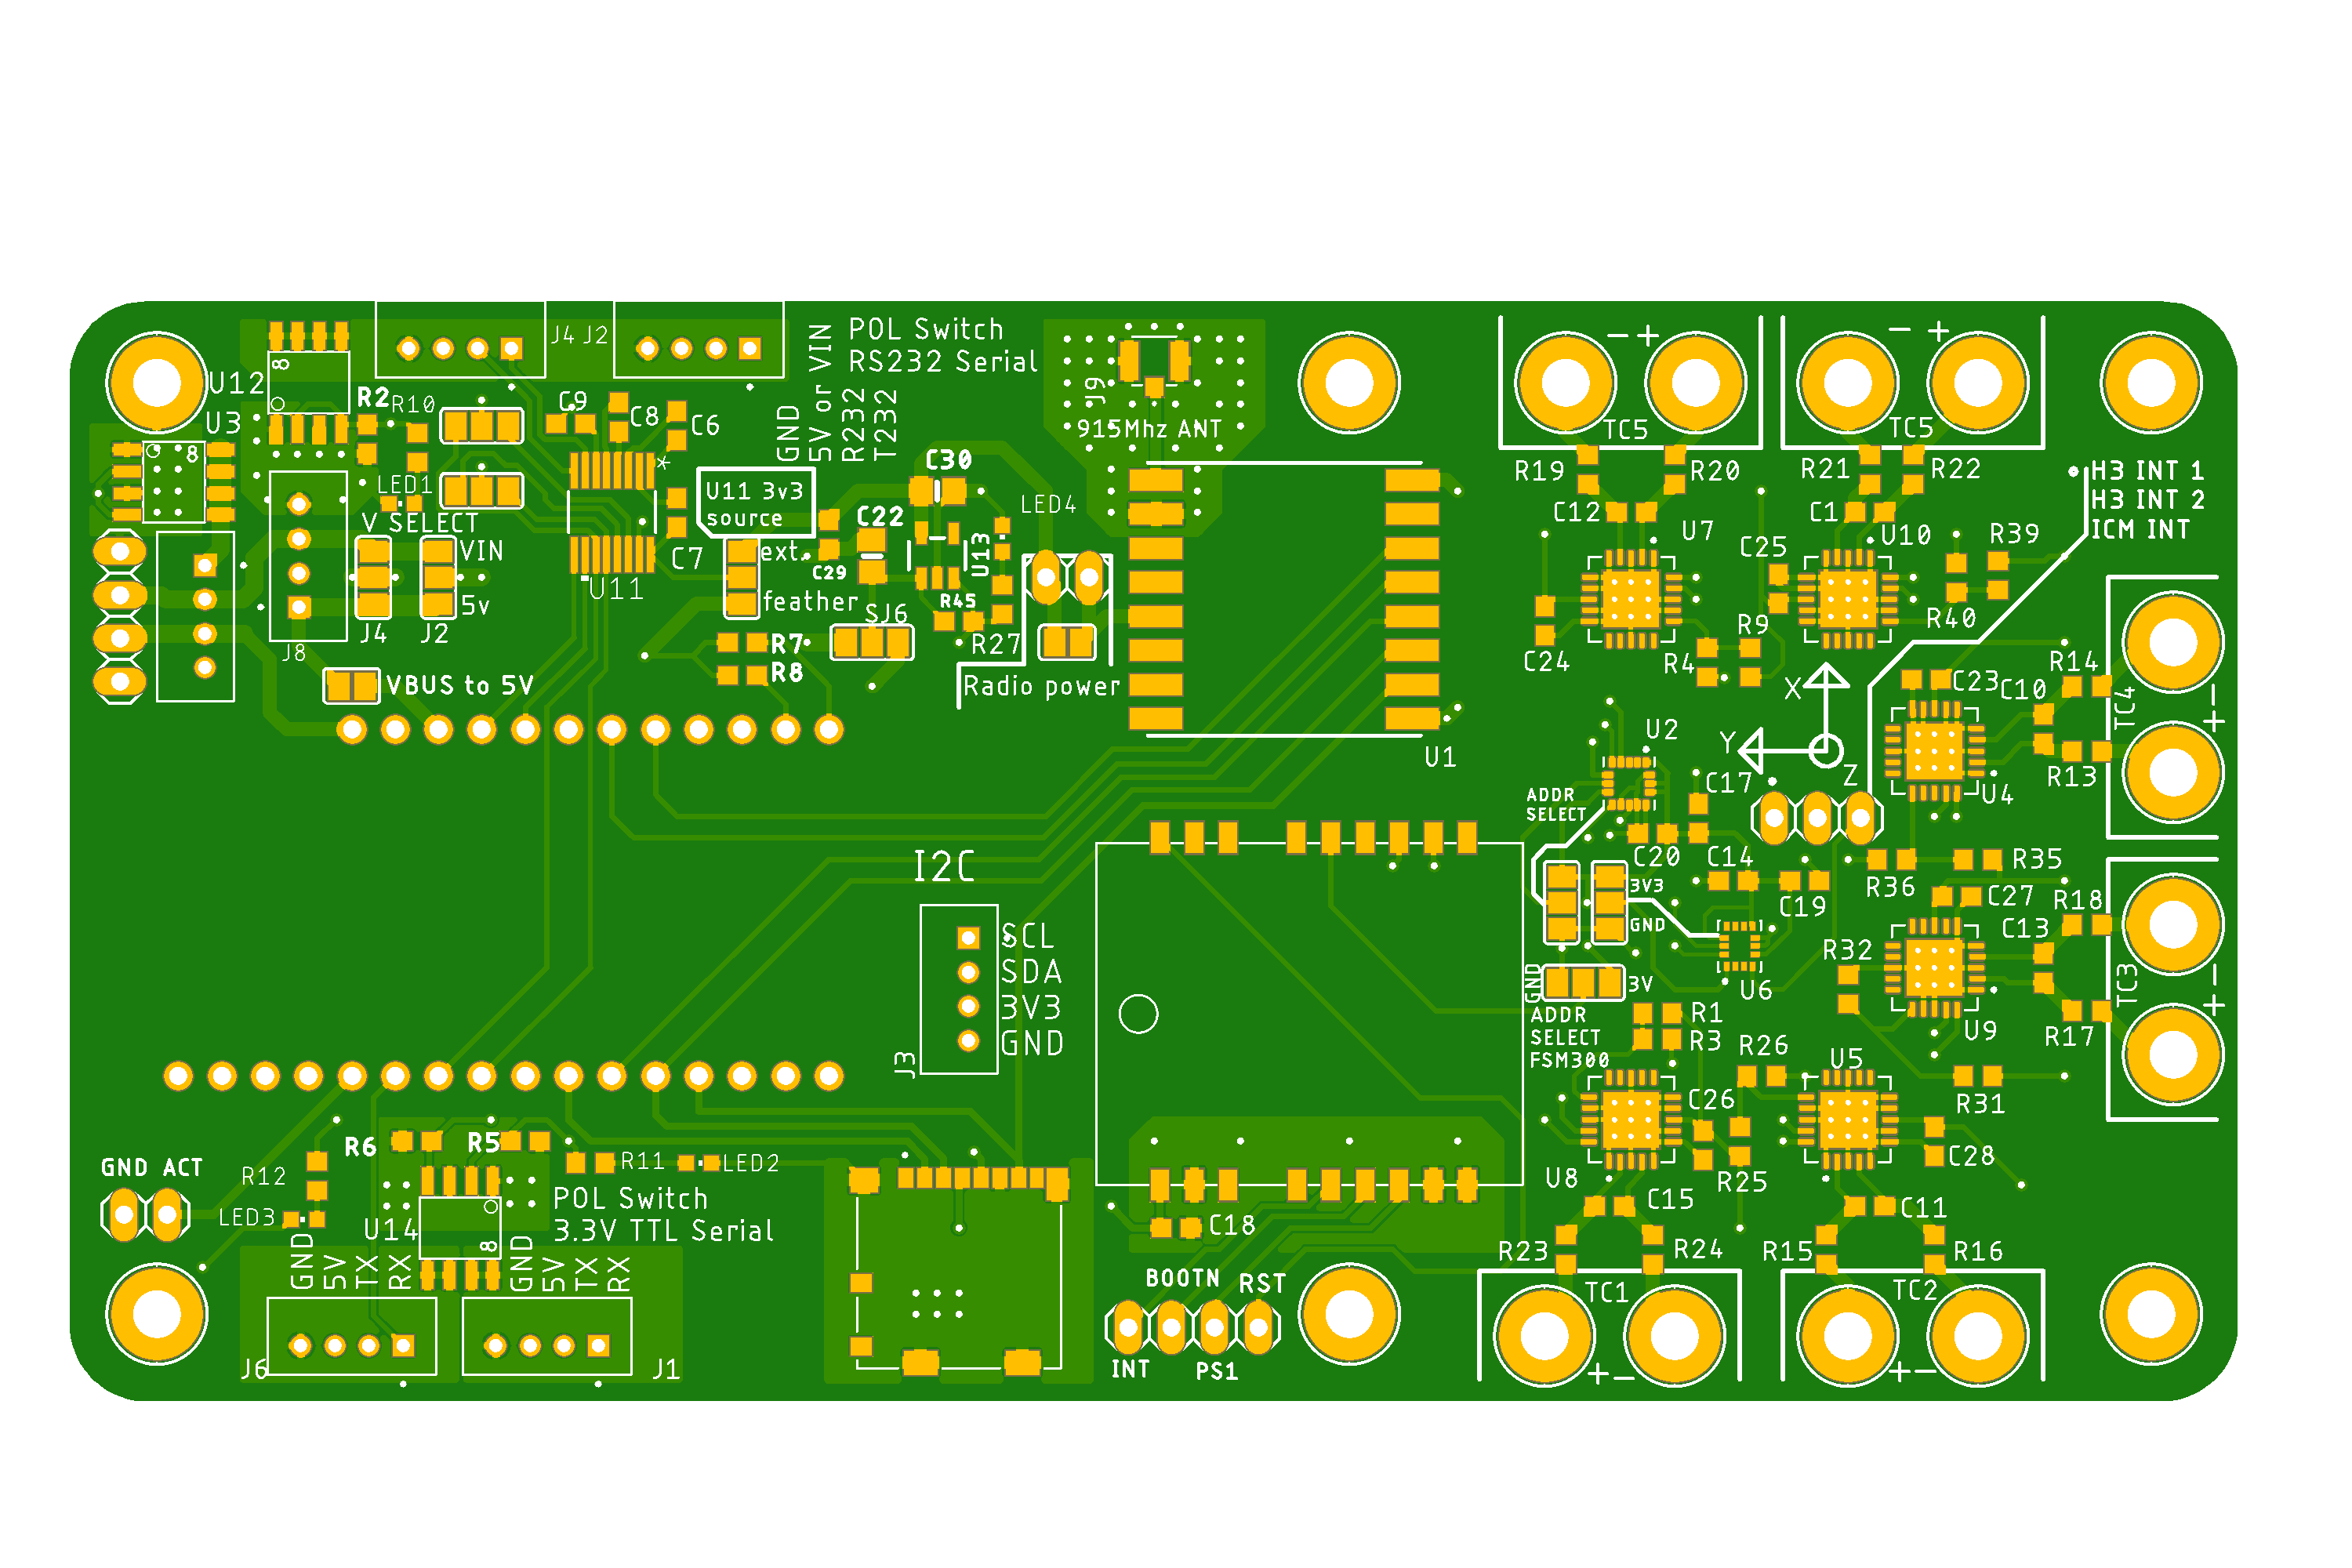
\includegraphics[width=0.9\textwidth]{images/main_board-top.png}
	\caption{Rendering of the top of the KREPE-2 control board.}
	\label{fig:board-top}
\end{figure}
\begin{figure}[H]
	\centering
	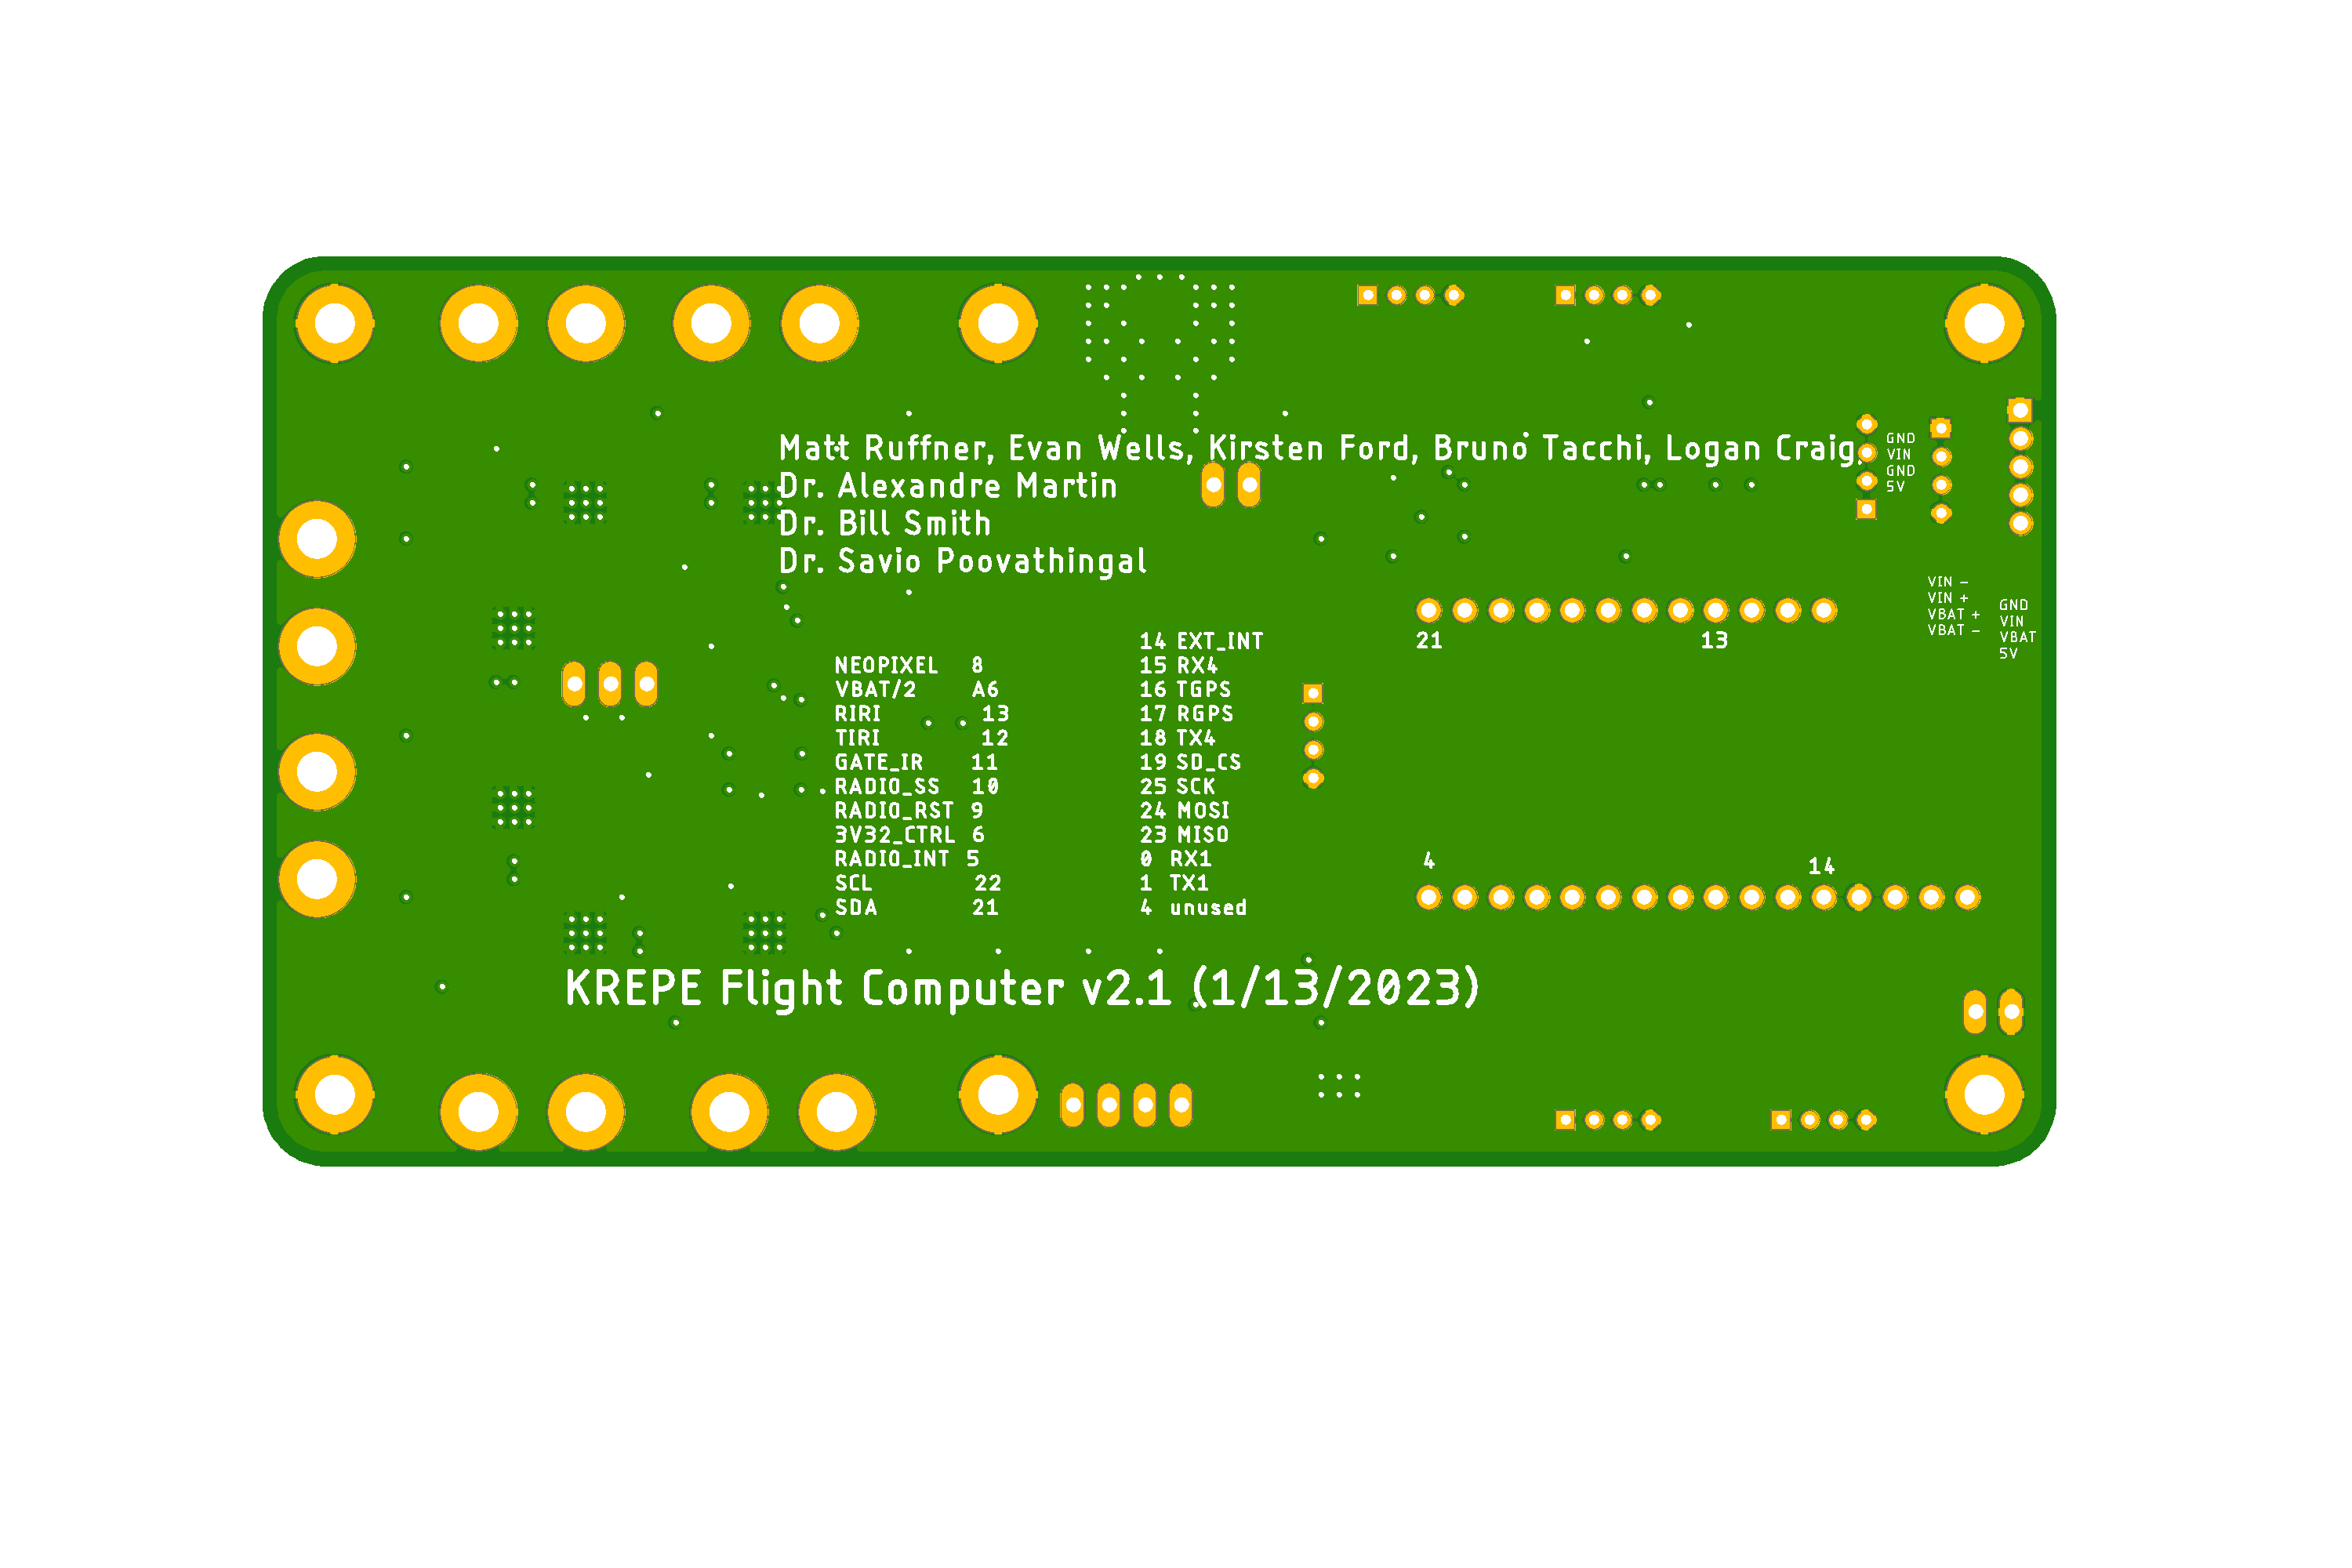
\includegraphics[width=0.9\textwidth]{images/main_board-bottom.png}
	\caption{Rendering of the bottom of the KREPE-2 control board.}
	\label{fig:board-bottom}
\end{figure}


%%%%%%%%%%%%%%%%%%%%%%%%
%%%%%%%%%%%%%%%%%%%%%%%%
\section{COTS hardware references}
This section contains reference cards for the COTS components used in the KREPE-2 capsules.
\subsection{Feather M4 Express}
\begin{figure}[H]
    \centering
    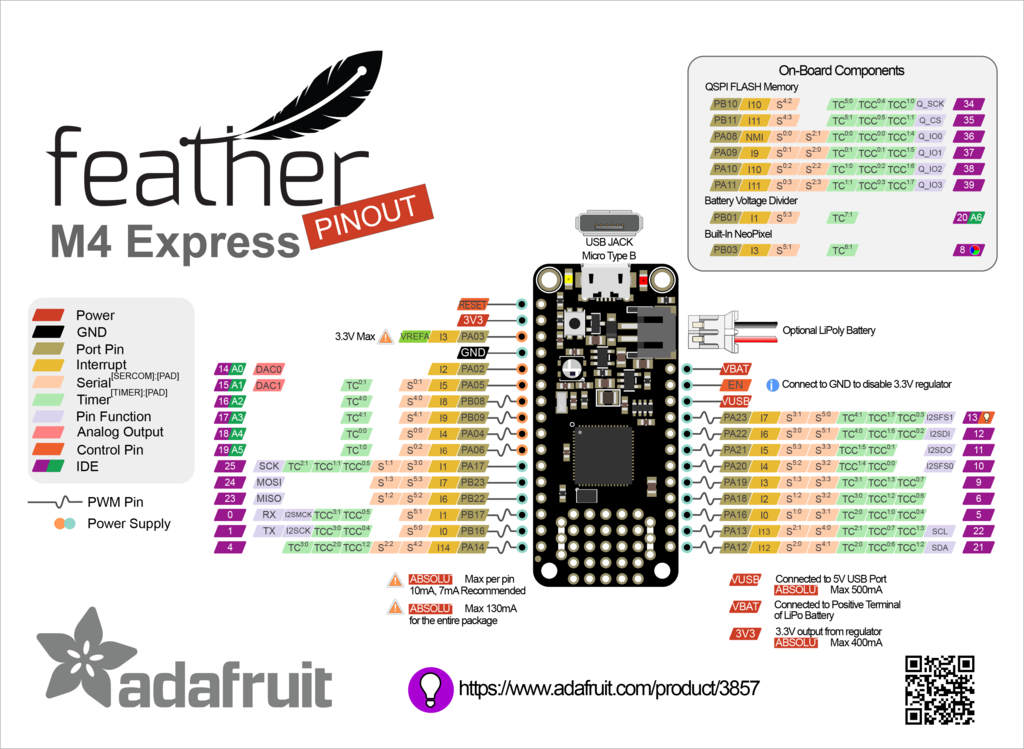
\includegraphics[width=\textwidth]{images/featherm4pinout.png}
    \caption{Feather M4 Express}
    \label{fig:teensy-front}
\end{figure}

\subsection{Nano Pi Neo Air}
\begin{figure}[H]
    \centering
    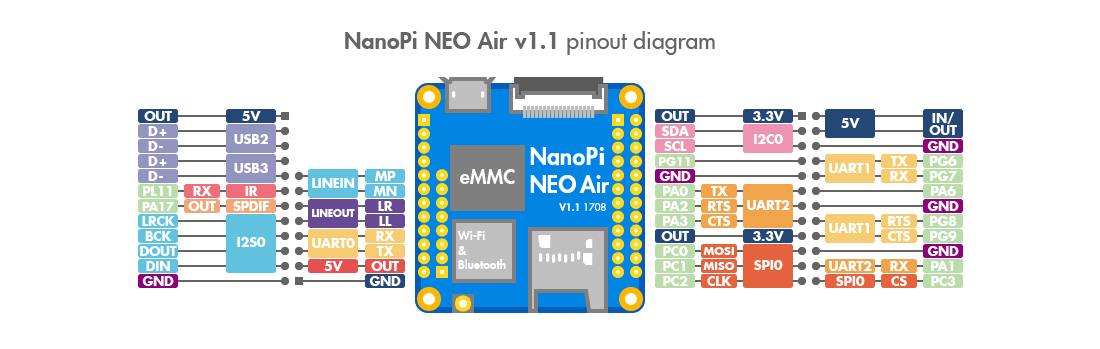
\includegraphics[width=\textwidth]{images/neo air pinout.jpeg}
    \caption{NanoPi Neo Air reference sheet.}
    \label{fig:trinket-m0}
\end{figure}


\section{Partslist}
\label{app:partslist}
\lstinputlisting[language={},basicstyle=\tiny]{flight-computer-partslist.txt}

%%%%%%%%%%%%%%%%%%%%
%%%%%%%%%%%%%%%%%%%%
%%%%%%%%%%%%%%%%%%%%
\newpage
\section{Arduino Pin Mapping}
\label{app:pinmap}
\lstinputlisting[language={}]{arduino-pinmap.txt}

%\bibliographystyle{plain}
%\bibliography{references}
\end{document}
